\section{Experiments}
\label{sec:experiments}
%%%%%%%%%%%%%%%%%%%%%%%%%%%%%%%%%%%%%%%%
%%%%%%%%%%%%%%%%%%%%%%%%%%%%%%%%%%%%%%%%%%%%%%%%%%%%%%%%%%%%
\begin{figure*}[t]
%%%%%%%%%%%%%%%%%%%%
\begin{minipage}[b]{0.29\linewidth}
               \centering
%%             \small
%              \begin{tabular}{l|rr|rr|}
%              (D10,                                                  T10)                                    & Naive                        (5M)                                     & Mahif                      (5M)                          & Naive                        (50M)                                          & Mahif                      (50M) \\ \cline{1-5}
%              U10                                                    & 125.587s                              & 8.145s                       & 1423.456s                              & 90.187s                    \\
%              U20                                                    & 121.911s                              & 8.467s                       & {\color{red}                           time                         out                           (30m)}                         & 90.513s                                      \\
%              U50                                                    & 277.642s                              & 10.448s                      & {\color{red}                           time                         out                           (30m)}                         & 84.611s                                      \\
%              U100                                                   & 502.570s                              & 18.761s                      & {\color{red}                           time                         out                           (30m)}                         & 116.525s                                     \\
%              U200                                                   & 1263.736s                             & 74.494s                      & {\color{red}                           time                         out                           (30m)}                         & 194.292s
%              \end{tabular}
               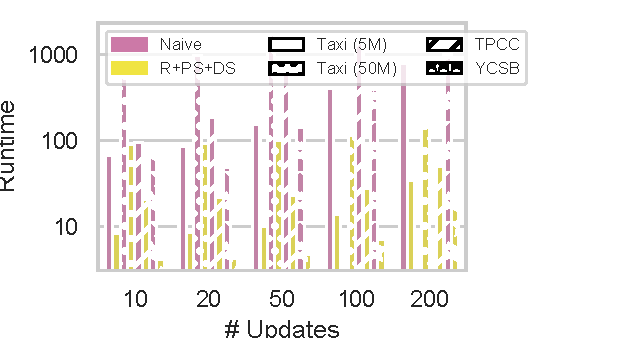
\includegraphics[width=1.1\linewidth,trim=0            0 0                                     0,                             clip]{imgs/felix_naive.pdf}              \\
               \vspace{-4mm}
               \caption{Naïve                                         vs.                                     Mahif                          (sec)}
               \label{fig:Naive                                       vs                                      Mahif}
               \end{minipage}
               %%%%%%%%%%%%%%%%%%%
%%%%%%%%%%%%%%%%%%%%
               \begin{minipage}[b]{0.35\linewidth}
               \centering
               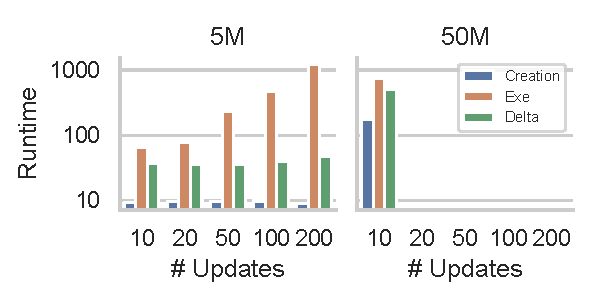
\includegraphics[width=0.95\linewidth,trim=0 8 0                                     0,                             clip]{imgs/felix_naive_breakdown.pdf}    \\
               \vspace{-3mm}
               \caption{Breakdown Naïve}
               \label{fig:Naive Method}
               \end{minipage}
%%%%%%%%%%%%%%%%%%%%
\begin{minipage}[b]{0.34\linewidth}
\centering
               % \scalebox{0.8}{
%              \scriptsize
%              \begin{tabular}{|r|rrrr|rrrr|}
%              \hline
%              & \multicolumn{4}{c|}{\textbf{5M}}                     & \multicolumn{4}{c|}{\textbf{50M}}     \\
%              \hline
%              \rotatebox{90}{\textbf{Updates}}                       & \rotatebox{90}{\textbf{PS}}           & \rotatebox{90}{\textbf{Exe}} & \rotatebox{90}{\textbf{R+PS+DS}}       & \rotatebox{90}{\textbf{R}} & \rotatebox{90}{\textbf{PS}} & \rotatebox{90}{\textbf{Exe}} & \rotatebox{90}{\textbf{R+PS+DS}$\,$$\,$$\,$} & \rotatebox{90}{\textbf{R}} \\
%              \hline
%              10                                                     & 0.07                                  & 8.08                         & 8.14                                   & 63.63                      & 0.07                        & 90.11                        & 90.18                                        & 722.23                     \\
%              20                                                     & 0.18                                  & 8.29                         & 8.47                                   & 81.12                      & 0.18                        & 90.33                        & 90.51                                        & 878.70                     \\
%              50                                                     & 1.30                                  & 9.15                         & 10.45                                  & 133.29                     & 1.29                        & 83.32                        & 84.61                                        & 1414.94                    \\
%              100                                                    & 8.46                                  & 18.76                        & 27.23                                  & 218.87                     & 8.46                        & 108.07                       & 116.53                                       & 2310.84                    \\
%              200                                                    & 62.13                                 & 12.36                        & 74.49                                  & 400.71                     & 62.22                       & 132.07                       & 194.29                                       & 4173.17                    \\
%              \hline
%              \end{tabular}
%              }
               \resizebox{1\linewidth}{!}{
               \begin{tabular}{|ll|rrrrr|}
               \hline
               &                                  &                   \multicolumn{5}{c|}{\textbf{\#Updates}} \\
               \textbf{Size}                                          & \textbf{Method}                       & \textbf{10}                  & \textbf{20}                            & \textbf{50}                & \textbf{100}                & \textbf{200}                 \\                                             \hline
               %
               \multirow{4}{*}{\textbf{5M}}                           & PS                                    & {{1}}                         & {{2}}                                   & {{3}}                       & {{4}}                        & {{5}}                        \\
               & Exe                                                  & {{6}}                                  & {{7}}                         & {{8}}                                   & {{9}}                      & {{10}}                       \\
               & R+PS+DS                                              & {{11}}                                  & {{12}}                         & {{13}}                                  & {{14}}                      & {{15}}                       \\
               & R                                                    & {{16}}                                 & {{17}}                        & {{18}}                                 & {{19}}                     & {{20}}                      \\                             \hline
               \multirow{4}{*}{\textbf{50M}}                          & PS                                    & {{21}}                         & {{22}}                                  & {{23}}                       & {{24}}                        & {{25}}                        \\
               & Exe                                                  & {{26}}                                 & {{27}}                        & {{28}}                                  & {{29}}                     & {{30}}                      \\
               & P+PS+DS                                              & {{31}}                                 & {{32}}                        & {{33}}                                  & {{34}}                     & {{35}}                      \\
               & R                                                    & {{36}}                                & {{37}}                       & {{38}}                                & {{39}}                    & {{40}}                     \\
               \hline
               \end{tabular}
               }                                                                                                                                                                                                                                                                                                               \\[-4mm]
               %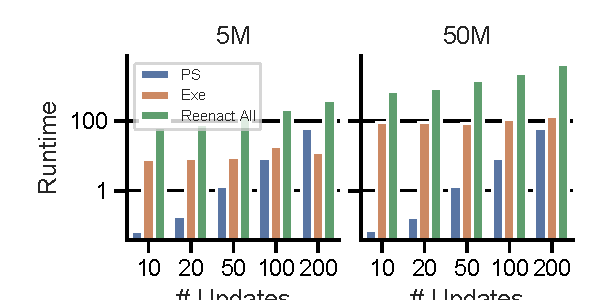
\includegraphics[width=0.95\linewidth,trim=0          0 0                                     0,                             clip]{imgs/felix_mahif_breakdown.pdf}    \\
               \caption{Breakdown                                     Mahif}
               \label{fig:Mahif                                       Method}
\end{minipage} \\
%%%%%%%%%%%%%%%%%%%%%
               \begin{minipage}[b]{0.245\linewidth}
               \centering
               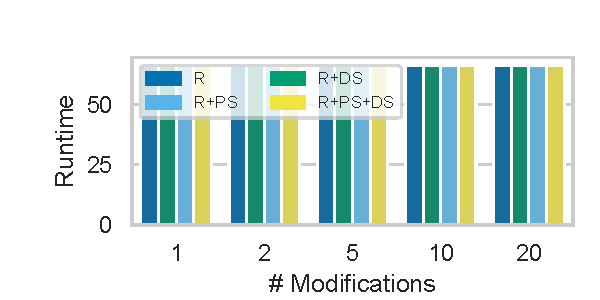
\includegraphics[width=0.95\linewidth,trim=7 5 0                                     0,                             clip]{imgs/felix_multimod.pdf}           \\
               \vspace{-3mm}
               \caption{Mult. Modifications}
               \label{fig:Multimod}
\end{minipage}
%%%%%%%%%%%%%%%%%%%%
\begin{minipage}[b]{0.275\linewidth}
               \hspace{-0.4cm}
               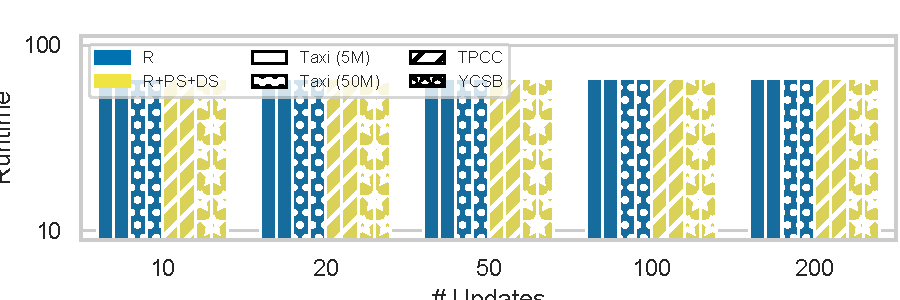
\includegraphics[width=1.2\linewidth,trim=0            0 0                                     0,                             clip]{imgs/felix_optimizations.pdf}      \\
               \vspace{-8mm}
               \caption{Optimization}
               \label{fig:optimization}
               \end{minipage}
%%%%%%%%%%%%%%%%%%%%%
               \begin{minipage}[b]{0.235\linewidth}
               \hspace{2mm}
               \scalebox{1}{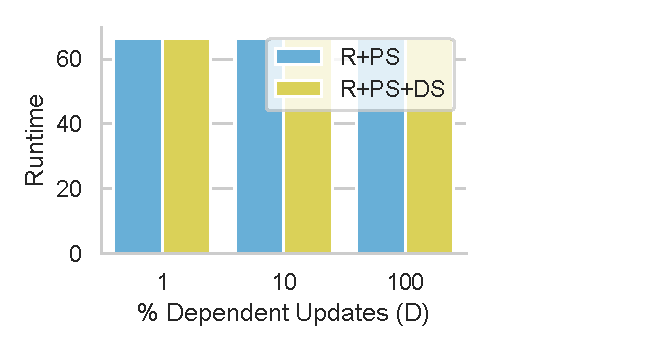
\includegraphics[width=1.0\linewidth,trim=22 0 50pt                                  0,                             clip]{imgs/felix_dependent_updates.pdf}} \\
               \vspace{-8mm}
               \caption{Dependent Updates}
               \label{fig:Dependent Updates}
               \end{minipage}
%%%%%%%%%%%%%%%%%%%%%
               \begin{minipage}[b]{0.225\linewidth}
               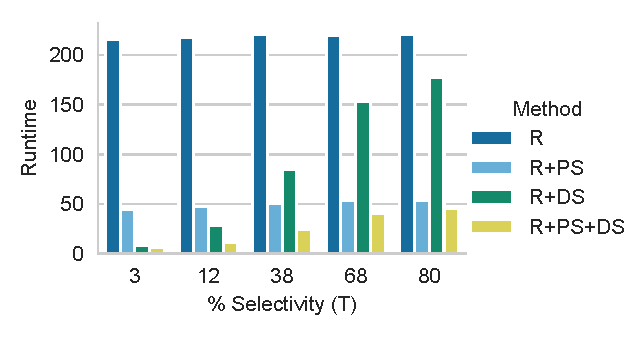
\includegraphics[width=1\linewidth,trim=0              0 0                                     0,                             clip]{imgs/felix_affected_data.pdf}      \\
               \vspace{-8mm}
               \caption{Affected                                      Data}
               \label{fig:Affected                                    Data}
               \end{minipage}                                         \\
%%%%%%%%%%%%%%%%%%%%
%              \begin{minipage}[b]{0.245\linewidth}
%              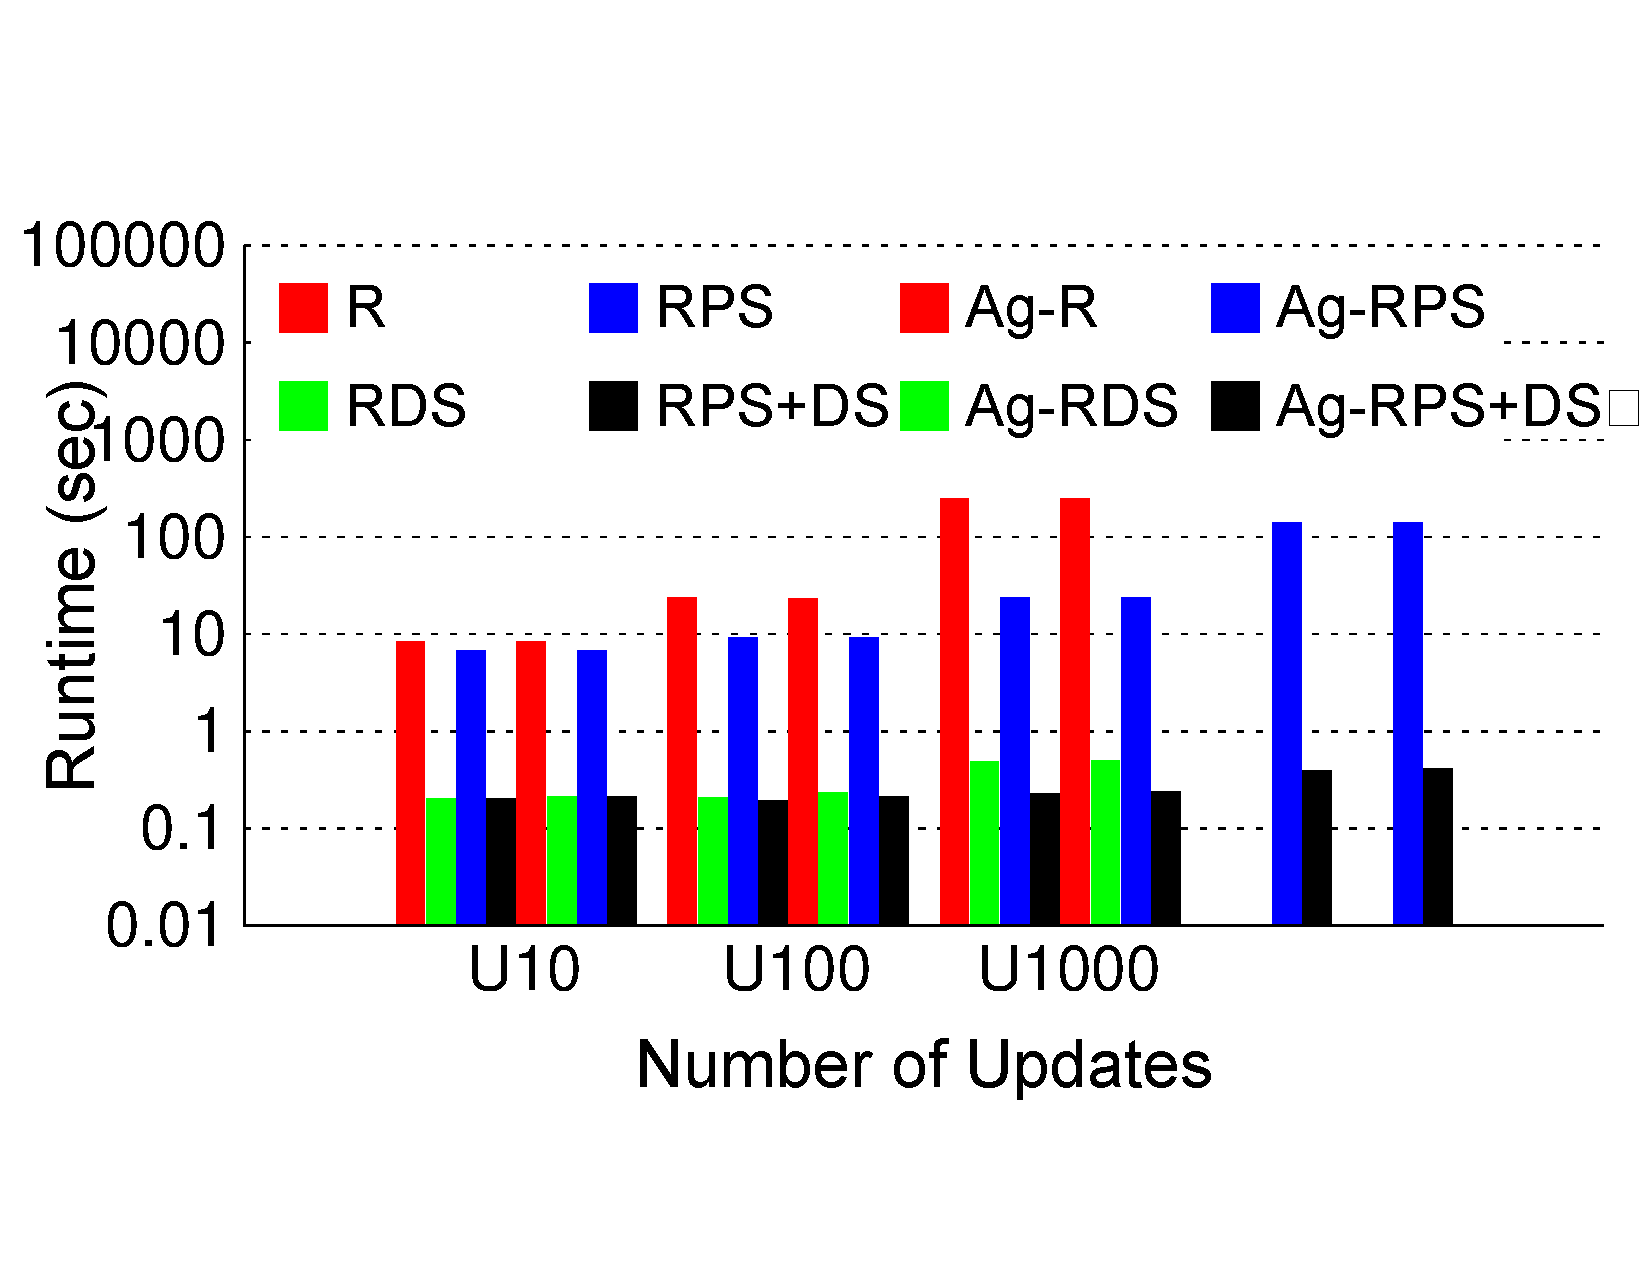
\includegraphics[width=1\linewidth,trim=0              50pt                                    0 80pt,                        clip]{imgs/aggregation.pdf}              \\
%              \vspace{-6mm}
%              \caption{Aggregation}
%              \label{fig:aggregation0}
%              \end{minipage}
%%%%%%%%%%%%%%%%%%%%%
\end{figure*}

%%% Local Variables:
%%% mode: latex
%%% TeX-master: "historical_whatif"
%%% End:


\newcommand{\mn}{\textit{N}\xspace}
\newcommand{\mr}{\textit{R}\xspace}
\newcommand{\mrd}{\textit{R+DS}\xspace}
\newcommand{\mrp}{\textit{R+PS}\xspace}
\newcommand{\mrdp}{\textit{R+PS+DS}\xspace}

%%%%%%%%%%%%%%%%%%%%%%%%%%%%%%%%%%%%%%%%
%%%%%%%%%%%%%%%%%%%%%%%%%%%%%%%%%%%%%%%%
%\begin{figure}[t]
%%%%%%%%%%%%%%%%%%%%%
%  \begin{minipage}[b]{0.49\linewidth}
%  \includegraphics[width=1\linewidth,trim=0 50pt 0 80pt, clip]{updates.pdf}
%  \vspace{-6.5mm}
%  \caption{Updates/Transaction}
%  \label{fig:Updates-Trans}
%  \end{minipage}
%%%%%%%%%%%%%%%%%%%%%
%  \begin{minipage}[b]{0.49\linewidth}
%  \includegraphics[width=1\columnwidth,trim=0 50pt 0 80pt, clip]{depen.pdf}
%  \vspace{-6.5mm}
%  \caption{Dependent Updates}
%  \label{fig:Depend-Trans}
%  \end{minipage}
%%%%%%%%%%%%%%%%%%%%%
%\end{figure}
%%%%%%%%%%%%%%%%%%%%%%%%%%%%%%%%%%%%%%%%
\BG{In general it would be good to have more descriptive figure captions}
We have conducted experiments to 1) evaluate the performance of our approach and compare it with the naïve approach, 2) examine the effectiveness of the proposed optimizations, and 3) study how our approach scales in database size and % evaluate how the performance of our approach is affected by
other important factors.\BG{What factors? Let's be specific}
All experiments were performed on a machine with 2 x AMD Opteron 4238 CPUs (12 cores total), 128 GB RAM, and 4 x 1TB 7.2K
HDs in a hardware RAID 5 configuration. We used PostgreSQL 11.4 as the database backend.
%Transactions were executed under the snapshot isolation concurrency control protocol~\cite{BB95}.
Based on preliminary experiments, the variance of runtimes was determined to be low. We repeated each experiment at least 3 times and report average runtimes.
%Our current implementation does not support multiple modifications.
%\FC{add error bars}
% the  2) study how our proposed algorithm scales in the number of operations.
% We have evaluated our system
% in two sets of experiments. In the
% first set of experiments we

%%%%%%%%%%%%%%%%%%%%%%%%%%%%%%%%%%%%%%%%%%%%%%%%%%%%%%%%%%%%
\subsection{Datasets and Workloads}\label{sec:exp-data-and-workloads}
%%%%%%%%%%%%%%%%%%%%%%%%%%%%%%%%%%%%%%%%%%%%%%%%%%%%%%%%%%%%%%%%%%%%%%%%%%%%%%%%
\partitle{Datasets}
We use a taxi trips dataset from the Chicago's open data portal \footnote{https://data.cityofchicago.org/Transportation/Taxi-Trips/wrvz-psew (2020-10-13)}, as well as the standard TPC-C \footnote{TPC-C is an On-Line Transaction Processing Benchmark: http://www.tpc.org/tpcc/} and YCSB~\cite{CooperSTRS10} benchmarks to evaluate the performance of our approach. % The taxi trip dataset contains trips reported to the City of Chicago.
The original taxi dataset has $\sim100$M rows and 23 attributes.
The dataset contains trip information such as the \texttt{Company} (the taxi company), the \texttt{Taxi ID}, \texttt{Trip Start Timestamp}
(when the trip started), \texttt{Trip Seconds} (duration of the trip in seconds), \texttt{Trip Miles}
(distance of the trip in miles), \texttt{Pickup Community Area}, \texttt{Tips}, \texttt{Tolls}, \texttt{Extras} (tips, tolls and extra charges for the trip), and \texttt{Trip Total} (total cost of the trip).
%
%As a data preparation step we removed tuples with NULL values in any of these columns.\BG{Resulting number of rows}.
%Data cleaning and data transformation was performed on the data for the purpose of our experiments. We removed removed tuples that have missing values in the aforementioned attributes. As a Taxi ID can be associated with any number of Company, we created a new \texttt{Company ID} attribute to uniquely identify taxis. % for each unique combination of Company and Taxi ID, to create a realistic and interesting aggregation.
%In order to extract a history with which we can make modifications to evaluate historical what-if queries, we aggregated the data grouping on Company ID, Community Area and Trip Start Timestamp and used aggregation functions (e.g. Sum, Min, Max, AVG and COUNT) over remaining attributes to create ten aggregated attributes like \texttt{Sum\_TripTotal} which is the sum of all \texttt{Trip Total} values for each group. Since we group on time, the result of this process can be interpreted as a temporal history of these aggregate statistics, e.g., how does the number of trips for a particular taxi to a particular community area change over time. When generating this temporal history table, we aggregated trip start time varying the temporal granularity (Month, Day, Hour). The resulting tables have $60K$, $200K$, and $600K$ rows.
% created three different tables based on the different granularity of trip start time (Month, Day, Hour). These tables have three grouping attributes (Company ID, Community Area and Trip Start Timestamp) using for grouping data and used aggregation functions (e.g. Sum, Min, Max, AVG and COUNT) over remaining attributes to create ten aggregated attributes like \texttt{Sum\_TripTotal} which shows sum of all \texttt{Trip Total} values for each group. These generated tables have three different sizes about $60K$, $200K$, and $600K$ rows based on the granularity of their \texttt{Trip Start Timestamp}.
% We created temporal tables for these three tables with a lower granularity of \texttt{Trip Start Timestamp} to simulate update operations that modify these tables to update their aggregated attributes.
We used samples from these tables amounting to 10\% ($5M$) and 50\% ($50M$) of the entire taxi dataset in some of the experiments. The TPC-C and YCSB benchmark databases were generated with OLTP-Bench \cite{DifallahPCC13}. For TPC-C, we used  the \texttt{stock} relation consisting of 10$M$ rows (scale factor 100).
 For YCSB database we used scale factor 5000, resulting in a single relation consisting of 5$M$ rows. The workloads generated by OLTP-Bench for each benchmark were modified to control the proportion of affected tuples.

%%%%%%%%%%%%%%%%%%%%%%%%%%%%%%%%%%%%%%%%%%%%%%%%%%%%%%%%%%%%%%%%%%%%%%%%%%%%%%%%
%For the aggregated history taxi tables, we generate a sequence of update operations to simulate a transactional history that aligns with the temporal history encoded in these tables.
%For instance, consider the history table with temporal granularity of months. If the total number of trips for community area 1 and company 1 increases by 10 from January 2013 to February 2013, then we would add the following update to the history to implement that change: \lstinline!UPDATE TAXI_TRIPS SET SUM_TRIPTOTAL ! \lstinline!= SUM_TRIPTOTAL + 10 ! \lstinline! WHERE COMPANYID=1 AND COMMUNITYAREAS=1 ! \lstinline! AND STARTDAY>=! \lstinline!20130101 AND STARTDAY<=20130121;!.
% Historical update operations are defined by a SET clause that assigns an attribute a relative value, and a WHERE clause has a point predicate on two categorical attributes and a range predicate on the trip start time attribute (e.g. \lstinline!UPDATE TAXI_TRIPS SET SUM_TRIPTOTAL ! \lstinline!= SUM_TRIPTOTAL + 10 ! \lstinline! WHERE COMPANYID=1 AND COMMUNITYAREAS=1 ! \lstinline! AND STARTDAY>=! \lstinline!20130101 AND STARTDAY<=20130103;!). These update statements are generated by \BG{Why did we do this? How does this correspond to the temporal history of the tables explained above. We need to say that we derived updated from the temporal snapshots}
%For the larger datasets that were generated as samples of the original taxi trip datasets instead of through temporal aggregation,
%and were tested with workloads that simulate data repairs, with the histories being sets of operations to repair the data, where the modifications made could be used to evaluate e.g. which repairs are most viable. \FC{?}

%SET Clause: WHERE Clause.
%Constant: SET (a_i=?), .. Point: WHERE a_j=? & ..
%Relative: SET (a_i=a_i+?) Range: WHERE a_j in [?,?+r] & ..
%%%%%%%%%%%%%%%%%%%%%%%%%%%%%%%%%%%%%%%%%%%%%%%%%%%%%%%%%%%%%%%%%%%%%%%%%%%%%%%%
\partitle{Workloads}
%
Unless stated otherwise, we use \abbrHWs with a single modification that modifies the first update in a history over a single relation.
We vary the following parameters. $U$ is the number of updates in the history (e.g. $U100$ for 100 updates). % Operations in the history that operate over other relations are excluded.
$M$ is the number of modifications made to the history.
$D$ is the percentage of updates that are dependent on the update(s) modified by the historical what-if query. We use 10\% as the default  ($D10$).
%For instance, $D10$ and $U100$ means that 10 updates out of 100 updates in the history are dependent, i.e., only 10 updates have to be reenacted when using program slicing.
$T$ is the percentage of tuples in the relation that are affected by each dependent update (the default is 10\%), where $T0$ means that a small, constant number of tuples was affected. $I$ and $X$ are the percentage of statements in the history that are inserts and deletes, respectively.
% Historical what-if queries affect different number of tuples to adjust $D$ and $T$ variables.
Non-dependent statements affect a fixed fraction of the data equal to $T$, though independent from the tuples modified by dependent updates. % We do not control the amount of data affected by non-dependent updates in our experiments. % the historical what-if query.
%The default for percentage of modified tuples by the historical what-if query is 10\%.



%We use a single relation with five numeric
%columns with 1M tuples.
%%their values for these attributes were generated randomly using a uniform distribution. % with the
%% exception of the primary key attribute which is automatically
%% generated.
%We consider histories of 10 transactions where parameter $U$ is the number of update statements per transaction. % and $D$ is their percentage of updates dependent on the update modified by the what-if query.
%We consider what-if queries that modify a single update of the first transaction of a history. Each update statement affects 10 tuples which are chosen randomly based on a range condition over the primary key attribute (e.g., \lstinline!WHERE ID>30 AND ID<41!).
%UPDATE R SET B=100
%

%%%%%%%%%%%%%%%%%%%%%%%%%%%%%%%%%%%%%%%%
\subsection{Compared Methods}
We compare the following methods in our experiments.
\textbf{Naïve (N)}: This method creates a copy of the database as of the start time of the history which is modified by the what-if query (\texttt{Creation}), executes $\deltaHist$ over this copy (\texttt{Exe}), and then computes the delta $\iDiff{\history(\db)}{\history[\deltaHist](\db)}$ by running a query over the current database state and the updated copy (\texttt{Delta}).
\textbf{Reenactment Only (R)} creates a reenactment query for $\history$ and for $\ahmod$.
%For both queries we exclude statements that executed before the statement modified by the what-if query.
We use run both reenactment queries over the database, and then compute the delta. \textbf{Reenactment with Data Slicing (R+DS)}: same as \mr except that we restrict reenactment to the part of data that is determined to be relevant  by our data slicing optimization. \textbf{Reenactment with Program Slicing (R+PS)}: same as the \mr method except that we only reenact the subset of updates from a slice determined by our program slicing optimization. \textbf{Reenactment with Program Slicing + Data Slicing (R+PS+DS)}:  we apply both optimizations.

\Cref{fig:Naive vs Mahif} shows the naïve method's performance in comparison to \mrdp. \Cref{fig:optimization} shows the runtime of reenactment (\mr) and reenactment with all optimizations enabled (\mrdp).  \Cref{fig:Mahif Method} breaks down the cost of \mrdp into \texttt{PS} and \texttt{Exe}, and together they form the runtime of \mrdp which should be compared to the cost of \mr (\texttt{Reenact All}). Given the clear efficiency gains of \mrdp over \mn and \mr, we omit \mn and \mr from most remaining experiments and focus on evaluating our optimizations.
%For methods which use reenactment, heuristic relational algebra optimizations are activated~\cite{XN17}.

%GProM's heuristic and cost-based optimization framework
%as number of updates per transaction ($U$) and percentage of dependent in transactions ($D$).
% and 3) the overhead for transaction execution incurred by audit logging and history maintenance.
%A synthetic  workload  is used to analyze how this approach scales in various parameters and to compare two different isolation level \textit{SI} with $RC-SI$.
% the database size, the size of historical
% data, the number of updates per transactions, and the number of
% affected tuples per update.
% The second set of experiments uses a
% TPC-C based workload to confirm that these results translate to more
% realistic workloads.
% We also
% and measure the storage and runtime overhead of audit logging
% and history maintenance.
% for both the synthetic and the TPC-C workload.

%The runtime and storage overhead of DBMS X's build-in temporal and audit features were studied in~\cite{AG16}. The results demonstrated that the runtime overhead for transaction execution is below 20\%  when audit logging and time travel are activated and it is more efficient than eager materialization of provenance during transaction execution (about 133\% overhead and higher). We did confirm the same trend for RC-SI and, thus, do not present these results here.
%%%%%%%%%%%%%%%%%%%%%%%%%%%%%%%%%%%%%%%%
%%%%%%%%%%%%%%%%%%%%%%%%%%%%%%%%%%%%%%%%%%%%%%%%%%%%%%%%%%%%
\begin{figure*}[t]
%%%%%%%%%%%%%%%%%%%%
\begin{minipage}[b]{0.48\linewidth}
    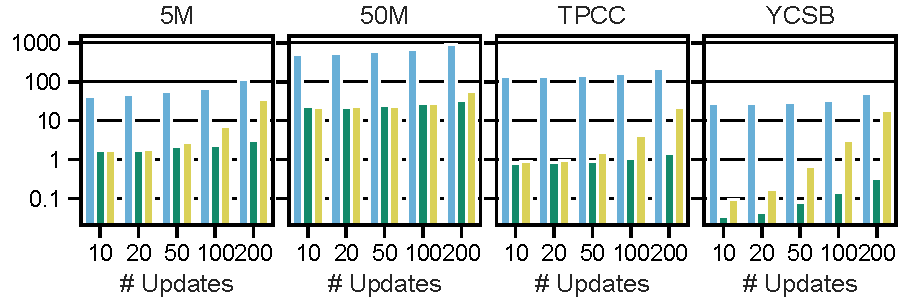
\includegraphics[width=1\linewidth,trim=0 0 0 0, clip]{imgs/felix_t0_optimizations.pdf}\\
    \vspace{-8mm}
  \caption{Datasets with T0}
  \label{fig:Relation Size}
  \end{minipage}
%%%%%%%%%%%%%%%%%%%%
 \begin{minipage}[b]{0.48\linewidth}
    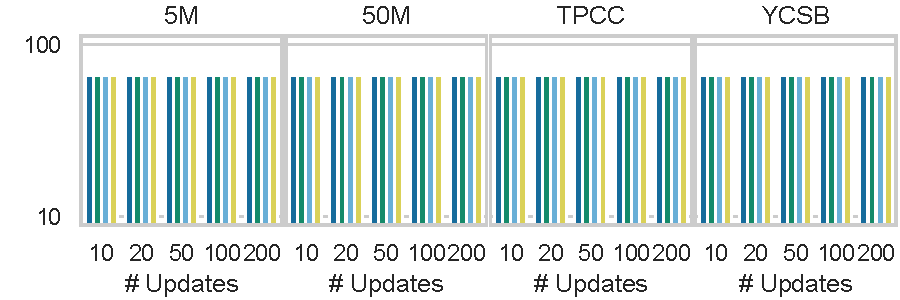
\includegraphics[width=1\linewidth,trim=0 0 0 0, clip]{imgs/felix_t10_optimizations.pdf}\\
    \vspace{-8mm}
  \caption{Datasets with T10}
  \label{fig:Relation Size1}
  \end{minipage}
  %%%%%%%%%%%%%%%%%%%%
\end{figure*}
\begin{figure}
  \begin{minipage}[b]{1\linewidth}
    $\,$\\[-5mm]
    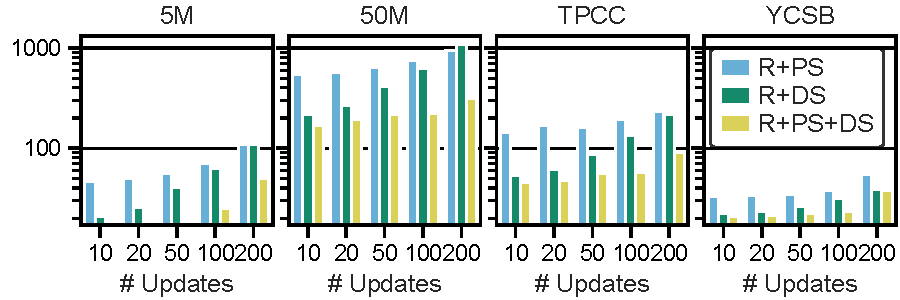
\includegraphics[width=1\linewidth,trim=0 0 0 0, clip]{imgs/felix_t25_optimizations.pdf}\\
    \vspace{-8mm}
  \caption{Datasets with T25}
  \label{fig:Relation Size2}
  \end{minipage}
%%%%%%%%%%%%%%%%%%%%
% %%%%%%%%%%%%%%%%%%%%%%%%%%%%%%%%%%%%%%%%
%% \begin{minipage}[b]{0.245\linewidth}
%%    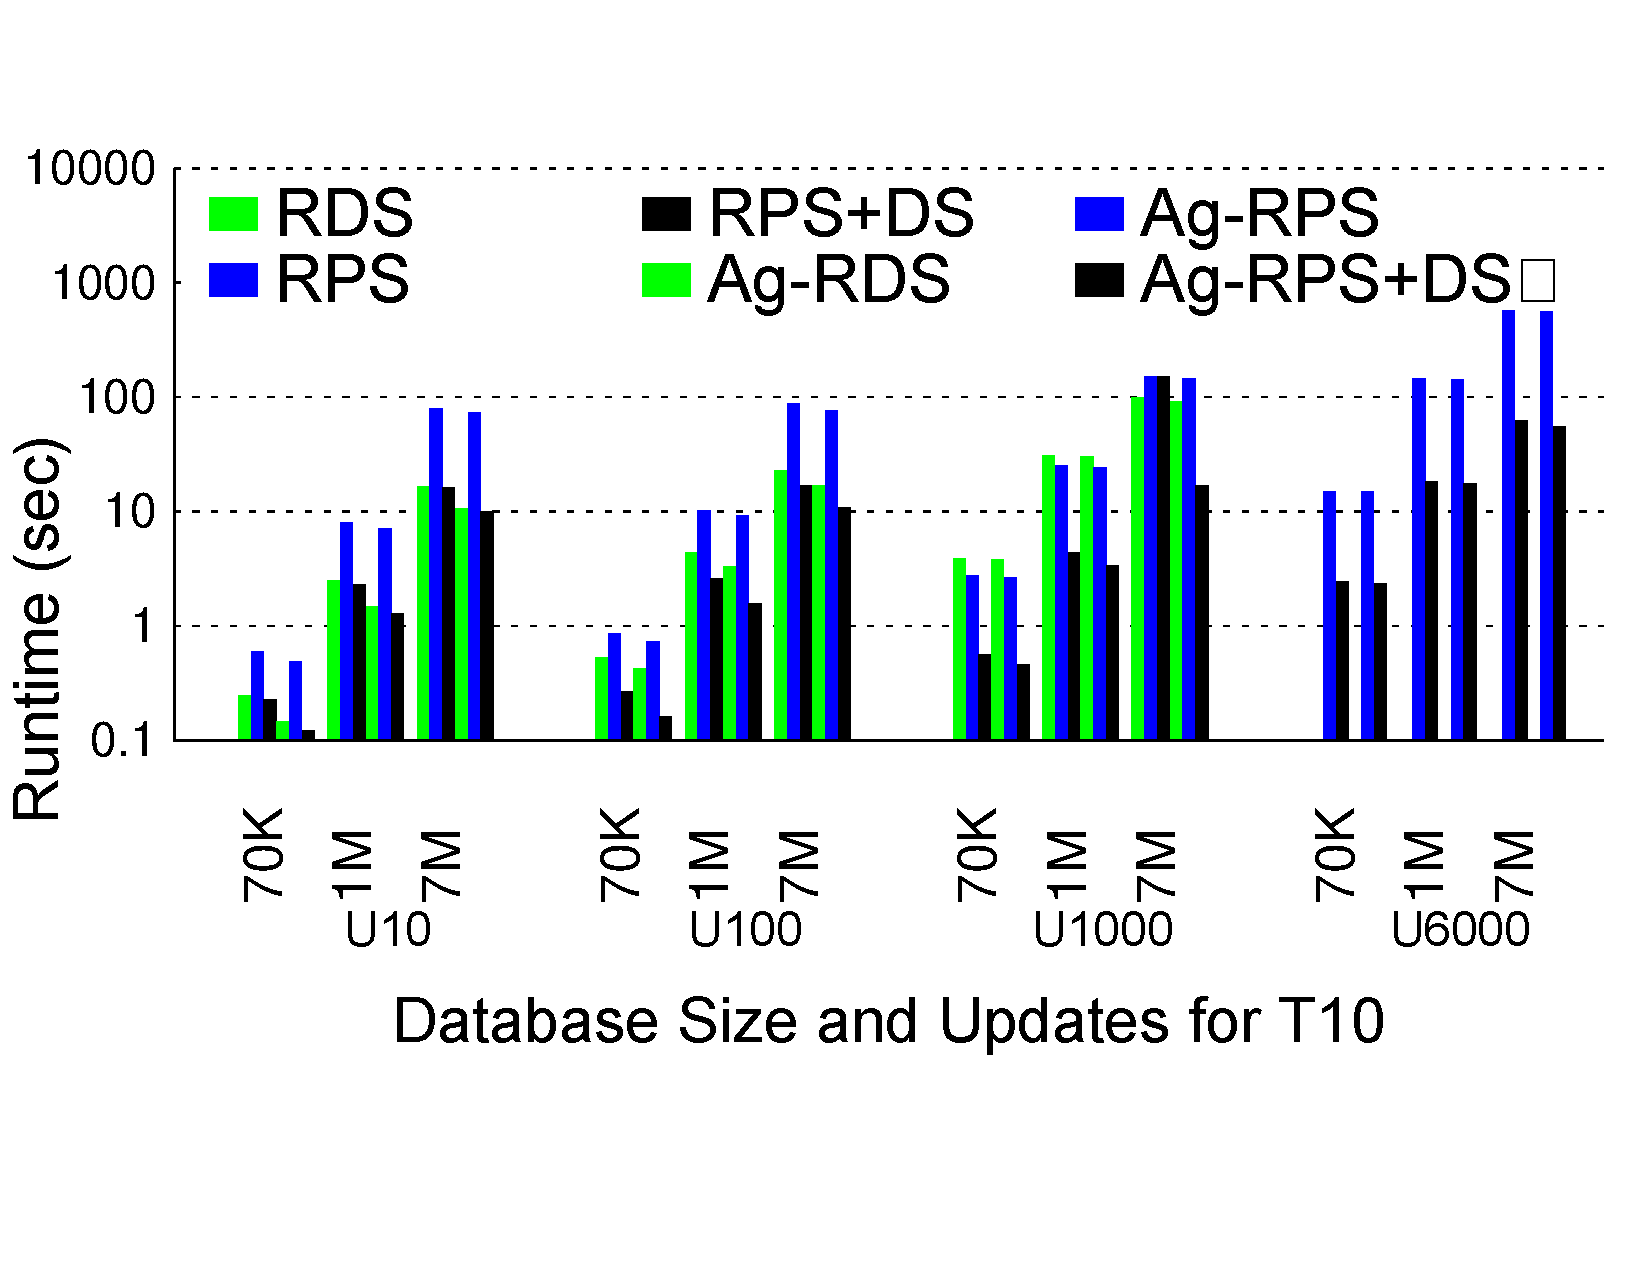
\includegraphics[width=1\linewidth,trim=0 50pt 0 80pt, clip]{imgs/agg10.pdf}\\
%%  \vspace{-6mm}
%%  \caption{Aggregate Query}
%%  \label{fig:aggregation0}
%%  \end{minipage}\\
%%%%%%%%%%%%%%%%%%%%
%   \begin{minipage}[b]{0.245\linewidth}
%    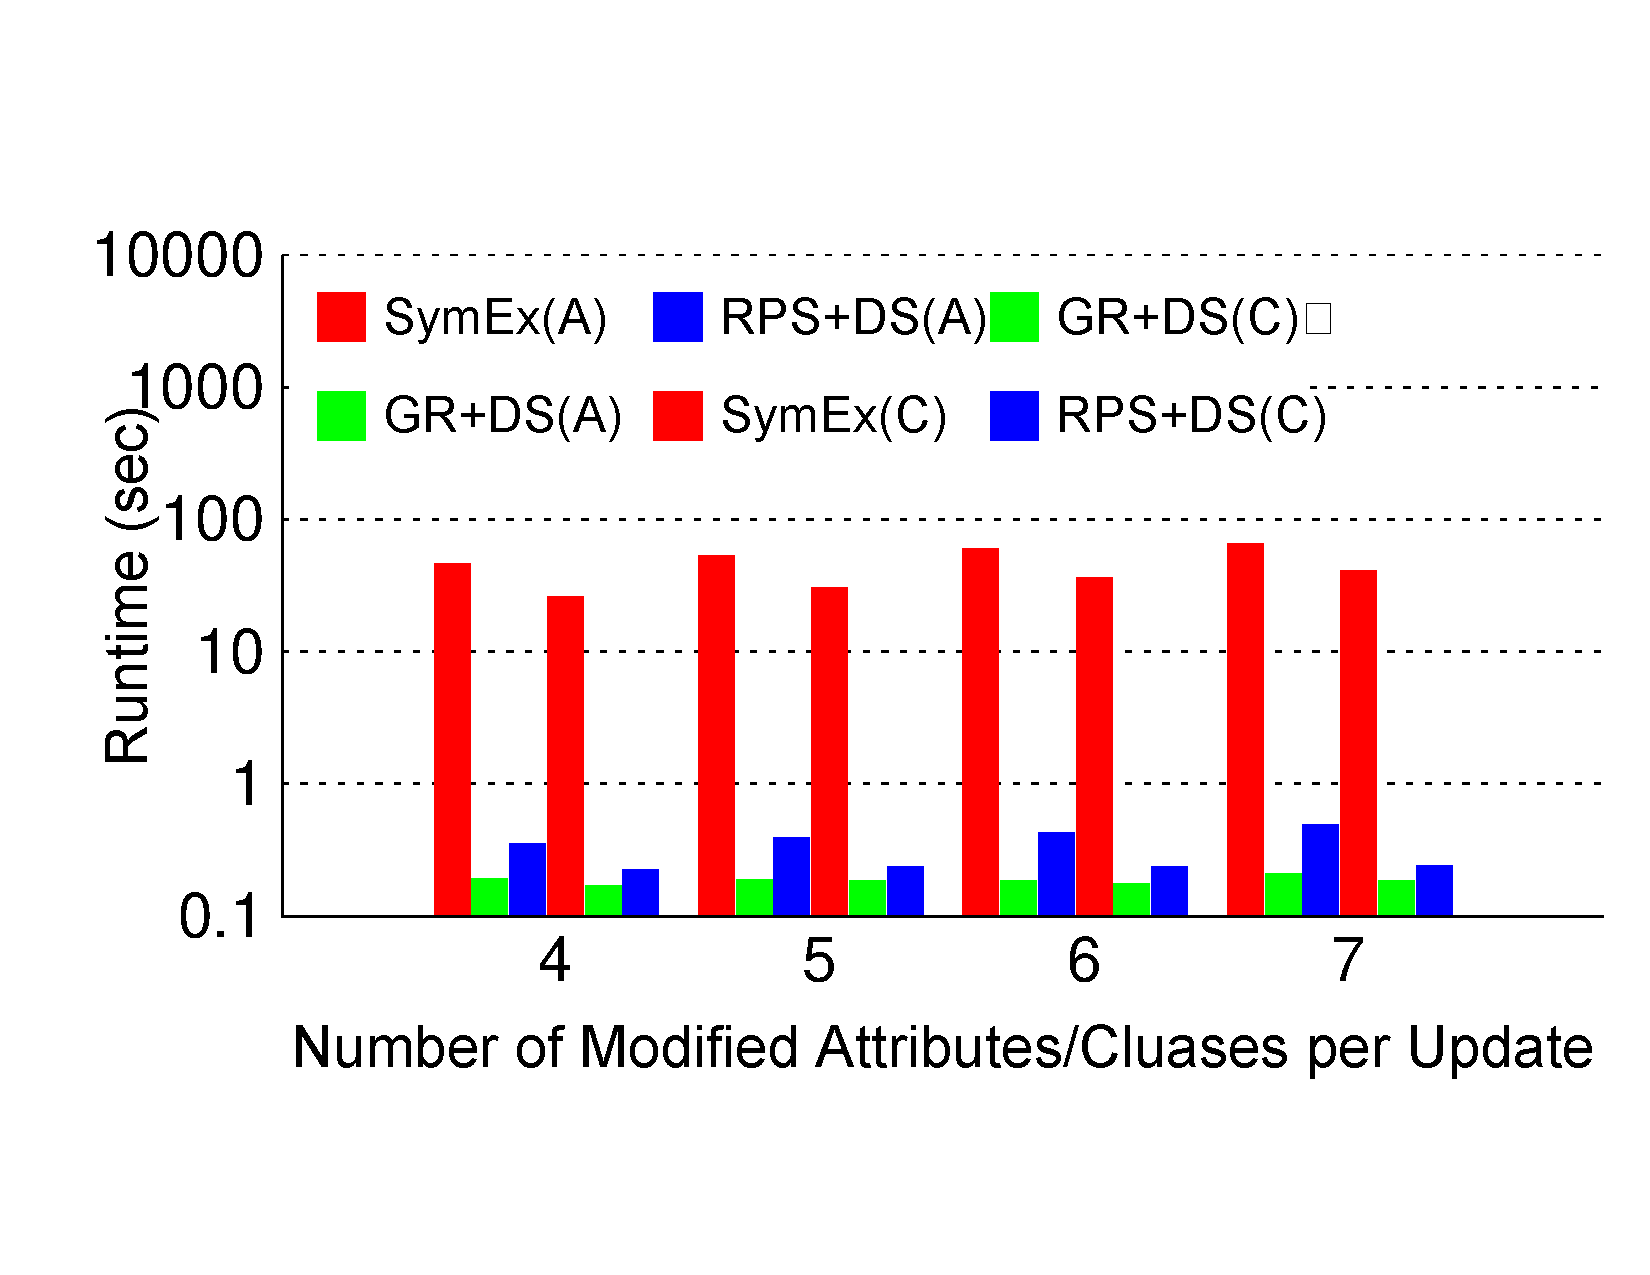
\includegraphics[width=1\linewidth,trim=0 50pt 0 80pt, clip]{imgs/attCla.pdf}\\
%  \vspace{-6mm}
%  \caption{Number of Attributes/Conditions}
%  \label{fig:Different Number of Attributes/Conditions}
%  \end{minipage}
%%%%%%%%%%%%%%%%%%%%
\end{figure}


%%% Local Variables:
%%% mode: latex
%%% TeX-master: "historical_whatif"
%%% End:

%%%%%%%%%%%%%%%%%%%%

%%%%%%%%%%%%%%%%%%%%%%%%%%%%%%%%%%%%%%%%
%%%%%%%%%%%%%%%%%%%%
\subsection{Optimization Methods}
We now evaluate our optimization techniques varying the parameters introduced in \Cref{sec:exp-data-and-workloads} over update-only workloads to observe which workload characteristics benefit which optimization.
%It is through these observations that we have derived certain insights as guidelines for when to enable or disable certain optimizations.

%\BG{The discussion in this part is a bit unstructured and does not serve the story line well. We should extract the major take-aways and then organize the structure around that. Maybe we can start with Figures 20-22 and then improve}


%%%%%%%%%%%%%%%%%%%%
\partitle{Varying Datasets (at D10)} %\label{sec:exp-relation-size}
We vary number of updates and amount of tuples affected per update ($T0$, $T10$, $T25$). Overall, we see that our approach scales very well in dataset size. As the cost of program slicing is independent of the database size, larger datasets benefit much more from program slicing. % For smaller datasets, program slicing has diminishing returns as the cost of program slicing may be more expensive than it would be to run \mr or \mrd over the entire history.
For lower selectivity (\Cref{fig:Relation Size}), we see that \mrd is very competitive with \mrdp for the smaller Taxi dataset (5M) as reenactment of the entire history over a small relation and an even smaller proportion of affected input data is cheaper than the cost of solving the MILP problem for program slicing. Notably, for the YCSB dataset, the MILP cost exceeds the cost of $\mrd$, as data slicing is well-served by the physical correlation of the key used to update the data. For larger proportions of data to be reenacted (\Cref{fig:Relation Size1} and \Cref{fig:Relation Size2}),  \mrdp  consistently outperforms \mrp and \mrd. The optimal case for \mrdp is when the size of the  affected input data as determined by data slicing is large enough that calculating and reenacting over a slice is worth the execution cost of the generated MILP.

%%%%%%%%%%%%%%%%%%%%

%\partitle{Varying Data Size and Number of Updates (at T10)}
%\BG{Add parameter abbreviation here, e.g., Affected Data (T)}
%\label{sec:exp-opt}

%Figure 14 demonstrates the effectiveness of our combined approach (reenactment, program \& data slicing) over the naïve method. The naïve method is significantly worse than our combined optimization method, with the closest gap in runtime being larger by a factor of 14 compared to R+PS+DS. Given this disparity, we omit results for the naïve method later as to focus on comparing our proposed optimizations. In Figure 17, reenactment alone is compared with reenactment with all optimizations enabled (R+PS+DS) by varying the data size and number of updates (tuple selectivity and proportion of dependent updates are fixed at 10\%). We see that the runtimes of R+PS+DS are consistently almost an order of magnitude less than reenactment alone.

%%%%%%%%%%%%%%%%%%%%%%%%%%%%%%%%%%%%%%%%%
\partitle{Varying Percentage of Dependent Updates (at T10)}
%\BG{Add parameter abbreviation here, e.g., Affected Data (T)}
\label{sec:exp-dep}
%
\Cref{fig:Dependent Updates} demonstrates the effect the proportion of dependent updates ($D$) in a given history has on \mrp, and how the addition of data slicing (\mrdp) is an effective way to mitigate these effects. This experiment uses the $5M$ row taxi trip table, with defaults T10 (10\% of tuples affected by modified updates) and U100 (100 updates in the history). As the proportion of dependent updates in the history increases, program slicing becomes less effective as more updates have to be included in the slice over the history. At D100 (100\% of updates are dependent), program slicing is not beneficial at all, but still incurs the MILP solver cost. However, data slicing  mitigates this effect, as the input to reenactment is filtered to include only a fraction of the data, making it more effective than \mrp at D100.

%%%%%%%%%%%%%%%%%%%%%%%%%%%%%%%%%%%%%%%%%
\partitle{Varying Affected Data (at U100, D1)}
\label{sec:exp-ds}
The effect of the percentage of  tuples affected by the updates modified by the \abbrHW ($T$) is examined in \Cref{fig:Affected Data}. This experiment is executed for 100 updates on the taxi trips relation with $5M$ rows. For example, $T3$ means 3\% of tuples ($\sim150$K out of 5M) are modified by the \abbrHW. The result demonstrates that varying $T$ does not change the performance of \mrp, as the whole history is evaluated over the full input table in all cases. However, increasing $T$, increases the runtime of \mrd and \mrdp considerably as data slicing becomes less efficient due to the greater amount of input data that needs to be accessed during reenactment. However, at moderate selectivity (T68), \mrdp provides enough filtering over the history and data to be more performant than either optimization alone. % The proportion of tuples affected by the dependent updates is therefore inversely proportional to the effectiveness of data slicing.
%
%Also, this experiment can represent how the performance of our methods are affected by increasing the number of tuples that are modified by each update in the history. The result would be similar as the number of tuples that must be processed would be increased. If each update modifies more tuples, then modified update in the historical what-if query and dependent updates also change more tuples.

%%%%%%%%%%%%%%%%%%%%%%%%%%%%%%%%%%%%%%%%
%%%%%%%%%%%%%%%%%%%%
%\subsection{Other Performance Variables}\BG{The section title is a bit too generic}
%\FC{cut? redundant (relation size in 15.3 \& no num. modified attributes)}
%In this section, we examine other variables which can affect the performance of our approach.

%%%%%%%%%%%%%%%%%%%%
%\partitle{Relation Size (at D10)}\BG{Add parameter abbreviation here, e.g., Affected Data (T)}
%\label{sec:exp-db-size}
%We vary the database size ($5M$, and $50M$) and the number of updates in the history ($U10$ to $U200$). We present the results %for our optimized methods for three different percentages of affected data.  $T0$ in \Cref{fig:Relation Size}, $T10$ in %\Cref{fig:Relation Size1}, and $T25$ in \Cref{fig:Relation Size2}. The result shows the runtime increases notably for higher $T$. %For all methods, we can see that the runtime scales with the amount of data being processed (related to both relation size and %$T$), demonstrating the effectiveness of data slicing to reduce the amount of data being evaluated. Additionally, this experiment %shows for higher number of updates in the history \mrdp runtime performance is better than \mrd alone. Given %that program slicing is data independent, it scales very well with an increase in data size where data slicing would otherwise %become ineffective. Its overhead is constant given the same amount of updates, and it can be seen from \Cref{fig:Affected Data} %that data slicing's effectiveness is inversely proportional to the amount of data selected by the data slicing condition.
%\BG{Either here or better earlier the fundamental trade-off for PS needs to be explained (data independent, constant over%head dependent on number of updates)}
%\FC{needs data update w/ new PS optimization}

% %%%%%%%%%%%%%%%%%%%%%%%%%%%%%%%%%%%%%%%%
%%%%%%%%%%%%%%%%%%%%%%%%%%%%%%%%%%%%%%%%
%\partitle{Inserts and Deletes}
%\label{sec:exp-ins-del}
%We now also use inserts and deletes
%in addition to updates...
% %%%%%%%%%%%%%%%%%%%%%%%%%%%%%%%%%%%%%%%%
%%%%%%%%%%%%%%%%%%%%%%%%%%%%%%%%%%%%%%%%
%\partitle{Number of Modified Attributes and Conditions}\BG{outdated}\FC{cut?}
%\label{sec:exp-num-mod}
%We examine the effect of increasing the number of modified attributes (\Cref{fig:Number of Attributes}) and  conditions in the %WHERE clause (\Cref{fig:Number of Conditions}) for each update in the history. We present results for $T0$, the relation with %$1M$ rows, and 1000 updates in the history. This experiment evaluates the runtime of each step in \textit{Mahif} similar to what %we present in \Cref{fig:Mahif Method}. \textit{SymEx} increases slightly by changing the number of modified attributes and %conditions from 4 to 7 as they increase the MILP problem complexity by adding new constraints. Increasing the number of %attributes that are modified by updates increases \textit{SymEx} more than extending the number of conditions of each update as %updating an attribute create a constraint recursively whereas adding new condition creates a simple new constraint. Note that  %\textit{RPS+DS} is faster in \Cref{fig:Number of Conditions} as adding conditions improves the data slicing method to filter more %data.


%%%%%%%%%%%%%%%%%%%%%%%%%%%%%%%%%%%%%%%%%%%%%%%%%%%%%%%%%%%%%%%%%%%%%%%%%%%%%%%%
\subsection{Mixed Workloads with Deletes and Inserts}\label{sec:mixed-workl-updat}

%%%%%%%%%%%%%%%%%%%%%%%%%%%%%%%%%%%%%%%%%
\begin{figure}[t]
  \begin{minipage}[b]{0.47\linewidth}
    \centering
		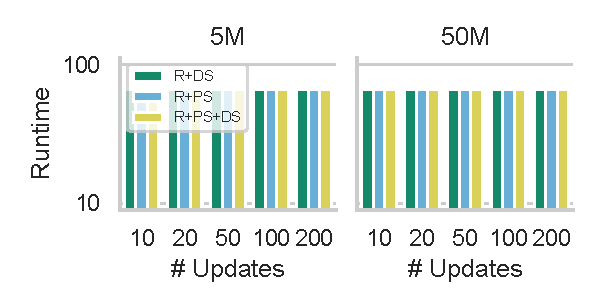
\includegraphics[width=1.1\linewidth,trim=10 9 15 10, clip]{imgs/felix_inserts.pdf}
		\vspace{-6.5mm}
		\caption{Inserts: I10, T10}
		\label{fig:Inserts at I10}
	\end{minipage}
	% %%%%%%%%%%%%%%%%%%%%%%%%%%%%%%%%%%%%%%%%
	\begin{minipage}[b]{0.52\linewidth}
      \centering
      \hspace{3mm}
      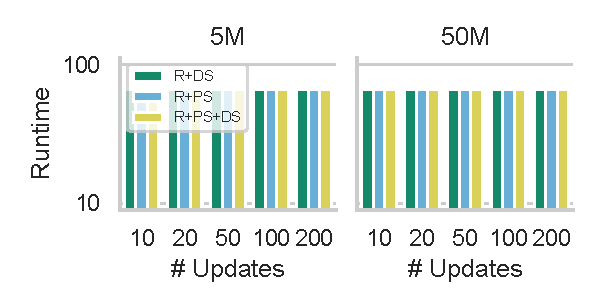
\includegraphics[width=0.9\linewidth,trim=30 9 15 10, clip]{imgs/felix_mixed.pdf}
		\vspace{-2.5mm}
		\caption{Mixed: I10, X10, T10}
		\label{fig:Mixed Updates at IX10}
	\end{minipage}
\end{figure}
%%%%%%%%%%%%%%%%%%%%%%%%%%%%%%%%%%%%%%%%

We now consider workloads that contain deletions, inserts, and updates. Since deletes are handled in a similar fashion to updates, we mainly focus on evaluating the impact of the fraction of inserts on performance. We use the taxi trip tables for this experiment. %to demonstrate the scaling factor across otherwise homogeneous tables.

As shown in \Cref{fig:Mixed Updates at IX10}, \mrdp outperforms the other methods for mixed workloads. When comparing to similar workloads presented in \Crefrange{fig:Relation Size}{fig:Relation Size2}, we see that introducing deletes and inserts into our workload in lieu of updates reduces the cost of reenactment and our optimizations. Note that delete statements result in fewer constraints in the program slicing MILP than update statements. Inserts are much cheaper to process than program slicing an update as we are able to reenact the unsliced prefix of the history on a very small amount of tuples (only the tuples being inserted, typically a very small fraction of a given workload).

%%%%%%%%%%%%%%%%%%%%%%%%%%%%%%%%%%%%%%%%%%%%%%%%%%%%%%%%%%%%%%%%%%%%%%%%%%%%%%%%
\subsection{Varying the number of modifications}\label{sec:vary-numb-modif}
So far we have evaluated \abbrHWs with a single modification. We now evaluate how multiple modifications affect the performance of Mahif and of the proposed optimizations.

\Cref{fig:Multimod} depicts the effect of changing the number of modifications per \abbrHW. Program slicing is more expensive than its single modification counterpart, given that we have to test each update by comparing the state of its symbolic tuple not only between $\history$ and $\ahmod$, but duplicating these histories while removing the update being tested, in order to not falsely classify an update as independent. This effectively quadruples the individual MILP program size over the single modification case. Data slicing also becomes more expensive as we employ the push down technique described in \Cref{sec:filter}, which in turn creates a selection operator with a  larger, more complicated condition. Recall that such selection conditions basically include some partial reenactment in order to capture every tuple that would be modified by modifications that occur after the first modification in the \abbrHW. That is, program slicing and data slicing are less efficient for multiple modifications.

The data from \Cref{fig:Multimod} shows a decrease in performance from a single modification to the multiple modification case. The nature of the modification (attributes updated, conditions, selectivity, dependencies across updates) significantly impacts the performance of \mrd, as evaluating the data slicing conditions pushed down through a long history is sometimes expensive. \mrdp remains an effective optimization compared to \mr, though its cost is higher than for single modifications. In part this is due to the effect of slicing the history which also reduces the size of conditions produced by pushing down  data slicing conditions. It should be noted that as the amount of modifications grows, the program slicing time goes down as these modifications are inherently dependent. That being said, an inflection point is possible where the gains in program slicing execution speedup results in a slowdown from the longer history the data slicing conditions need to be pushed through.
% In general, multiple modifications are most practical for lower selectivity, in order to provide the filtering that speeds up the execution of the slice.


% %%%%%%%%%%%%%%%%%%%%%%%%%%%%%%%%%%%%%%%%
%%%%%%%%%%%%%%%%%%%%
\subsection{Summary}
Our approach outperforms the naïve method in most cases despite it not needing any additional storage. Even reenactment without optimizations is already considerably faster than the naïve method.
The proposed optimizations are very effective, especially for large number of updates and larger databases. However, for small relations or very low selectivity, the cost of program slicing will outweigh the cost of reenactment or reenactment with data slicing. Data slicing is very effective for single modifications, but less so for multiple modifications, because the size and complexity of the data slicing conditions increases when these conditions are pushed through the updates upstream from a modification. Our experiments also show that our approach scales well with respect to database size.
%Factors like the query($\query$) type in a historical what-if query, number of modified attributes, or conditions of update operations do not affect the performance of our approach noticeably.
%%%%%%%%%%%%%%%%%%%%%%%%%%%%%%%%%%%%%%%%
%\partitle{Dependent Updates/Transaction}
%\label{sec:exp-vary-size-D}
%%fig:Depend-Trans
%In this experiment, we use 10 transactions with 100 updates ($U100$) and vary the number of updates that depend on the modified update from 1\% ($D1$) of the total number of updates up to 50\% ($D50$). The results are shown in
%\Cref{fig:Depend-Trans}.  We compare \textit{RPS+DS} and \textit{RPS}, the two methods that exploit dependencies. Both method's runtime increases with increasing number of dependencies.
%The performance of method \textit{RPS+DS} is dominated by the cost of time travel for this workload and, thus,
% % result demonstrates the importance of prefiltering input data as \textit{RD+P} performance is dominated by and, thus,
%reducing the number of updates that have to be reenacted has a less pronounced effect.
%%%%%%%%%%%%%%%%%%%%%%%%%%%%%%%%%%%%%%%%
%\BA{?}
%\partitle{Benchmark}
%\label{sec:exp-bench}
%%fig:Depend-Trans
%The performance of the answering historical what-if queries algorithm
%using data slicing and program slicing on the TPC-C and TATP benchmark
%applications.

% %%%%%%%%%%%%%%%%%%%%%%%%%%%%%%%%%%%%%%%%
%%%%%%%%%%%%%%%%%%%%%%%%%%%%%%%%%%%%%%%%
%\partitle{Updates/Transaction}
%\BA{its same as different history size}
%\label{sec:exp-vary-size-U}
%In this experiment we vary the number of updates per transaction ($U1$, $U10$, and $U100$). For instance, $U10$ denotes a history consisting of 10 transactions with 10 updates each.
%The runtimes of the different methods for answering a historical what-if query are shown in \Cref{fig:Updates-Trans}. Our fully optimized method \textit{RPS+DS} has the best performance outperforming the second best method (\textit{C}) by a factor of $\sim$ 3. The cost of \textit{C} is dominated by creating the copy of the input database and computing the delta while reexecuting the history has negligible cost ($\sim$ 0.5s for U100). For \textit{RPS+DS} the cost is dominated by the cost of time travel.
%%
%% The runtime of the  \textit{RD+P} and \textit{C} methods have a stable performance regardless of large number of update statements in transactions and .
%The large number of update statements in transactions considerably degrades the performance of the \textit{RPS} method that does not use data prefiltering and the \textit{RA} method which has to reenact all updates. While the cost of reenactment itself is tolerable, computing the delta over two large intermediate results is costly.
%% We compute different method \textit{C}
%%($\sim$ 2s)

% %%%%%%%%%%%%%%%%%%%%%%%%%%%%%%%%%%%%%%%%

%%% Local Variables:
%%% mode: latex
%%% TeX-master: "historical_whatif"
%%% End:
